\documentclass[14pt, a4paper]{extreport}
\usepackage{susu}

% ====================================================================================================
\begin{document}

\author{Савонин~М.В.}
\group{211}
\task{7}
\maketitle

% ====================================================================================================
\chapter{Задание}

\begin{enumerate}

	\item
	Написать программу для построения гладкой кривой по четырем опорным точкам. При выборе опорных точек текущие координаты указателя мыши 	должны отображаться в графическом окне. Интерфейс программы должен содержать следующие элементы управления:
	\begin{itemize}
		\item выбор опорных точек;
		\item построение кубической кривой Безье;
		\item построение кривой по алгоритму Чайкина;
		\item сохранение результата в файл;
		\item выход из программы.
	\end{itemize}

\end{enumerate}

% ====================================================================================================
\chapter{Математическая модель}

Класс Figure с полями:\\
px[3] = (20, 0, 0)\\
py[3] = (0, 20, 0)\\
pz[3] = (0, 0, 20)\\
figure[30] массив точек для отрисовки\\
\\
Методы класса:\\
Figure() конструктор, извлекает точки и полигоны\\
rote() вращает фигуру\\
move() двигает фигуру\\
draw() отрисовывает фигуру\\
\\
Матрица точек:\\
\begin{equation*}
\left(
\begin{array}{cccc}
0 & 0 & 70\\
114 & 37 & -50\\
70 & -97 & -50\\
-70 & -97 & -50\\
-114 & 37 & -50\\
0 & 120 & -50
\end{array}
\right)
\end{equation*}
\\
Матрица полигонов:
\begin{equation*}
\left(
\begin{array}{cccc}
0 & 1 & 2\\
0 & 2 & 3\\
0 & 3 & 4\\
0 & 4 & 5\\
0 & 1 & 5\\
1 & 2 & 3\\
3 & 4 & 5\\
1 & 3 & 5
\end{array}
\right)
\end{equation*}

% ====================================================================================================
\chapter{Текст программы}

\noindent Файл main.cpp
\lstinputlisting{source/main.cpp}
\pagebreak
\hrulefill

\noindent Файл task.h
\lstinputlisting{source/task.h}
\hrulefill

\noindent Файл task.cpp
\lstinputlisting{source/task.cpp}
\hrulefill

\noindent Файл control.h
\lstinputlisting{source/control.h}
\hrulefill

\noindent Файл control.cpp
\lstinputlisting{source/control.cpp}

% ====================================================================================================
\chapter{Результат работы}

\begin{figure}[h!]
	\centering
	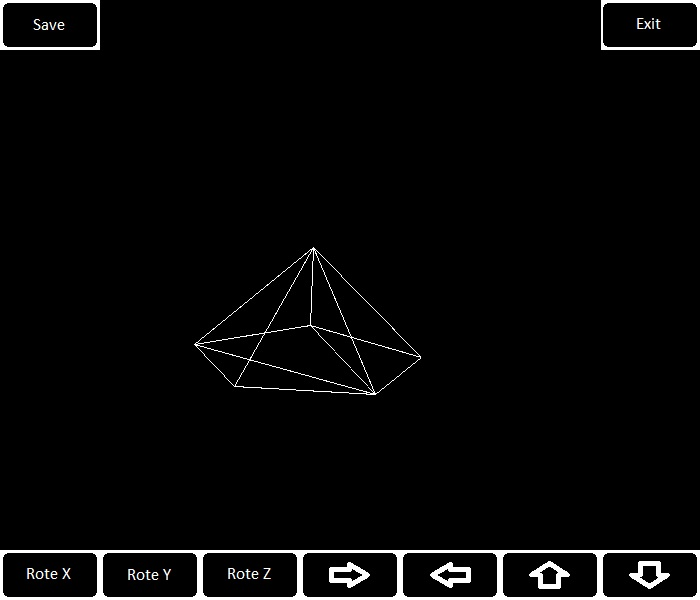
\includegraphics[width = 12cm]{image/output}
  \caption{Результат выполнения программы}
\end{figure}


% ====================================================================================================
\end{document}